%\documentclass[useAMS,usenatbib,preprint2]{aastex}
\documentclass{emulateapj}
% \documentclass[12pt,preprint]{aastex}
\usepackage{graphicx}
\usepackage{subfigure}
\usepackage{epsfig}
\usepackage{times}
\usepackage{natbib}
\usepackage{amsfonts}
\usepackage{amsmath}
\usepackage{amsbsy}

\bibliographystyle{apj}

%%%%%%%%%%%%%%%%

\begin{document}
\title{Intermittency of the 625 Hz QPO in the 2004 Hyperflare by SGR 1806-20}
\author{Daniela Huppenkothen, Anna L. Watts}
\affil{Instituut Anton Pannekoek, University of Amsterdam, Amsterdam  1098 XH,
  The Netherlands}
\email{d.huppenkothen@@uva.nl}
\author{Yuri Levin}
\affil{Monash}

\begin{abstract}
ABSTRACT GOES HERE!
\end{abstract} 

\keywords{pulsars: individual (SGR 1806--20), stars:
  magnetars, stars: oscillations, X-rays: stars}
\section{Introduction}
\label{sec:introduction}
Asteroseismology is now firmly established as a precision technique for the study of stellar interiors. In this regard the detection of seismic vibrations from neutron stars was one of the Rossi X-ray Timing Explorer's most exciting discoveries, as neutron star seismology allows a unique view of the densest matter in the Universe. The vibrations, detectable as quasi-periodic oscillations (QPOs) in hard X-ray emission, were found in the tails of giant flares from two magnetars \citep{Israel05, Strohmayer05, Strohmayer06, Watts06}. Magnetars are highly magnetized neutron stars that exhibit regular gamma-ray bursts powered by decay of the strong magnetic field \citep{Thompson95}, and the rare giant flares thought to be associated with large-scale catastrophic magnetic field reconfiguration are apparently sufficiently energetic that they can set the entire star ringing. Searches are now underway for vibrations in the more frequent but less energetic smaller flares \citep{Huppenkothen13} (hopefully also Huppenkothen 14!). It was realised immediately after their discovery that seismic vibrations from magnetars could constrain not only the interior field strength (which is hard to measure directly) but also the dense matter equation of state \citep{Samuelsson07,Watts07}. Over the last few years there has been intense development of seismic oscillation models that include the effects of the strong magnetic field, superfluidity, superconductivity, and crust composition \citep{Levin06,Levin07,Glampedakis06,Andersson09,Steiner09,vanHoven11,vanHoven12, Colaiuda11,Gabler12, Gabler13, Passamonti13a, Passamonti13b}.   

The prevailing view is the QPOs, which have frequencies that lie in the range 18-1800 Hz, are associated with global magneto-elastic (most likely torsional/axial) oscillations of the star. The models have had some success in explaining the presence of long duration oscillations in the lower frequency band below 150 Hz. However the higher frequency oscillations have proven to be something of a headache. Particularly problematic is a 625 Hz oscillation observed in data sets from two different satellites in the tail of the SGR 1806-20 giant flare \citep{Watts06, Strohmayer06}.  Frequencies in this range are predicted naturally in models where the crust vibrates independently without coupling to the core of the star, where they can be identified with the first radial overtone of the crustal shear modes \citep{Piro05}.  However for the field strengths expected (and measured) for magnetars, this crust mode should be absorbed into the core Alfv\'en continuum on timescales ~10-100 ms \citep{vanHoven12, Gabler12}. This would reduce surface amplitude and the signal should die out rapidly. The data analysis, by contrast, suggested that this signal persisted for ~ 100s \citep{Strohmayer06}.

Various solutions to this problem have been explored. Attempts to explain it as a magnetically dominated oscillation associated with a turning point of the Alfv\'en continuum itself have proven difficult \citep{vanHoven11, vanHoven12}. Coupling of the torsional (axial) oscillations to polar modes may break the continua and allow other types of oscillation to persist \citep{Lander10, Lander11, Colaiuda12}. Taking into account effects associated with superfluidity may also be the answer. Superfluidity can move the continua such that damping is reduced \citep{vanHoven08, Andersson09, Passamonti13a} and may result in resonances between crust and core that could prolong mode lifetimes \citep{Gabler13, Passamonti13b}.  In this paper we examine an alternative possibility and instead revisit the data analysis method, which as it turns out was not well-suited to address the question of whether the properties of the 625 Hz signal are consistent with rapid decay on very short timescales.

To understand why, we need to review the data analysis procedures that were followed. The amplitude of the strongest signal found SGR 1806-20 giant flare, at 92 Hz, was found to be strongly dependent on rotational phase. The signals at other frequencies were identified by taking short segments (typically 30\% of a rotational cycle, which corresponds to 2.3 s for SGR 1806-20), of consecutive rotational cycles, and averaging together power spectra from these individual segments. Significance was estimated using standard procedures for averaged power spectra \citep{vanderKlis89}, with corrections for the deviation of noise powers from a pure Poisson distribution, particularly at low frequencies. Having identified a significant signal (as compared to the null hypothesis), start/end points and hence durations for a signal of a given frequency were estimated by adding or subtracting power spectra from segments of rotational cycles at the ends of sequence, and identifying the set for which significance was maximised. This method was adequate to identify signals that were significant compared to the null hypothesis. However it does not distinguish between a signal that is present at a constant low level throughout the relevant segment of every rotational cycle, and one that is present for a much shorter time in perhaps only a few non-consecutive rotational cycles in the sequence.

We would like to test the specific question of whether the data are consistent with a model where whenever the 625 Hz signal appears, it dies out on a timescale that is much shorter than the segment durations considered in the previous analysis. We allow the possibility that the signal may be excited several times during the tail of the giant flares (perhaps by aftershocks)\footnote{The possibility of excitation late in the tail of the flare is already supported by the fact that the strongest 92 Hz signal does not appear until about 100s into the tail.}. A secondary goal is therefore to determine how many times, and at what level, the such a signal must be excited to be consistent with the data if this is indeed possible. In this paper we therefore develop a more sophisticated analysis method that is tailored to address the specific question of whether the data are consistent with rapid die-out of the 625 Hz signal, and the conditions that must be met in terms of re-excitation for this to be the case. It is interesting to note that the possibility that the data might be consistent with a sequence of rapidly decaying pulses may explain their apparent coherence. The width of many of the signals, including the 625 Hz QPO, is consistent with what one would expect for an exponentially decaying but strictly periodic signal with a decay timescale shorter than 1s. The fact that this was inconsistent with the apparent durations was noted by \citet{Watts11}, and taken as evidence that the signals were genuinely quasi-, rather than strictly, periodic.

\section{Data Analysis}
\label{sec:analysis}

We include data sets from two different space telescopes in our analysis: The {\it Rossi} X-ray timing Explorer (RXTE), and the {\it Ramaty High Energy Solar Spectroscopic Imager (RHESSI)}. An overview of the RXTE data is given in \citep{Israel05}. Data was recorded in $\mathrm{Goodxenon_2s mode}$, allowing for time resolution up to $1 \, \mu \mathrm{s}$, high enough to study high-frequency QPOs.
Observations taken with {\it RHESSI} are detailed in \citep{Watts06}. Following their analysis, we only used photons recorded with the eight front segments of the telescope, which are largely uncontaminated by scattering in the back of the space craft. The high-frequency QPO is seen only in the energy range between $100 \, \mathrm{keV}$ and $200 \, \mathrm{keV}$, hence we filter for these energies. All data are barycentered, that is, corrected for the motion of the space craft through space to avoid systematic effects in the timing analysis.

For the RXTE data, we concentrated on the part of the light curve where the $625 \, \mathrm{Hz}$ QPO was originally found, from around $190\, \mathrm{s}$ after the onset of the flare to the end of the observation. This encompasses a total of $15$ rotational cycles of the neutron star. The {\it RHESSI} observations place the same QPO at a slightly different frequency ($626.5 \, \mathrm{Hz}$ as opposed to $625.5 \, \mathrm{Hz}$), and at an earlier time. For the latter, we search the range from $80\, \mathrm{s}$ to $225 \, \mathrm{s}$ from the onset of the flare, or equivalently 19 cycles.

We split each rotational cycle into a number $N_\mathrm{r}$ of overlapping segments of length $\delta t_{\mathrm{s}}$. For each of these segments, we computed the periodogram and extracted the power at the frequency where the QPO was observed. For each periodogram we tested the significance of the observed power against $N_{\mathrm{sim}}$ simulations, which are constructed in the following way.

As a first step, we smoothed out the light curve to a resolution of $0.01 \, \mathrm{s}$, or equivalently $100 \, \mathrm{Hz}$, ensuring that all possible variability at smaller time scales is eliminated from the data. We then interpolated back to the original time resolution used ($\delta t = 2.5 \times 10^{-5} \, \mathrm{s}$), and added Poisson noise to this smoothed light curve $N_{\mathrm{sim}}$ times. This represents the null hypothesis that the QPO is not present, and that any variability measured at $625 \, \mathrm{Hz}$ is solely due to photon counting noise in the detector. For each of our $N_{\mathrm{sim}}$ simulations, we performed exactly the same analysis as for the observed data. We can then compare the real powers we measured for a given segment to the distribution of simulated powers in that segment. Additionally, we can compare the maximum power observed at $625 \, \mathrm{Hz}$ for all segments in our observed data for the maximum powers at this frequency in the ensemble of simulated light curves. This allows us to construct a p-value for the significance of the observed maximum power to be consistent with the null hypothesis, i.e. pure noise. Note that a number of trials correction for the number of segments searches is automatically included, since we apply the same search procedure to the simulations.


In addition to testing all segments individually, we constructed phase-averaged periodograms in the following way. We match all periodograms belonging to segments that start at the same phase with each other. In order to construct the two-cycle average, we average the same phase bins for two consecutive cycles together, and again extract the power at the relevant frequency. We then do the same for the next cycle, and so on until we reach the end of the data under consideration. The result is a moving average over subsequent rotational cycles, where the averaged periodograms match in phase.
Similarly, we can construct three-cycle averages by combining peridoograms from three consecutive cycles, and so forth, until we average the maximum number of cycles in our particular data set. Note that in both cases, the observed (averaged) powers are not independent. The powers extracted from the individual periodograms are not independent, because segments overlap substantially in our analysis (by design). 
Similarly, powers in averaged periodograms are not independent both of neighbouring segments as well as phase-matched segments, since each power is averaged at least twice with either neighbour (or more times in the case of constructing averaged periodograms from a larger number of rotational cycles). 
In each case, we apply the same analysis to our simulations, and thus construct averaged periodograms in the same way for each of our $N_\mathrm{sim}$ simulations. Consequently, we can construct simple p-values for the significance of a signal in the averaged periodograms. 
 

\section{Results}
\label{sec:results}

\subsection{RXTE}
\label{sec:rxte_results}

We repeated the analysis from \citealt{Strohmayer06}, paying special attention to the overall number of cycles during which the signal was present, as well as the duration of the presence of the QPO in any individual cycle.
We search individual segments of $3 \, \mathrm{s}$ length, starting every $0.5 \, \mathrm{s}$, such that consecutive segments overlap by $2.5 \, \mathrm{s}$. We extracted the power at $625 \, \mathrm{Hz}$, then ran 30000 simulations as described in \ref{sec:analysis} and compared the powers at $625 \, \mathrm{Hz}$ for each segment as well as phase-averaged segments to the powers extracted in the same way from the simulations.

\begin{figure*}[htbp]
\begin{center}
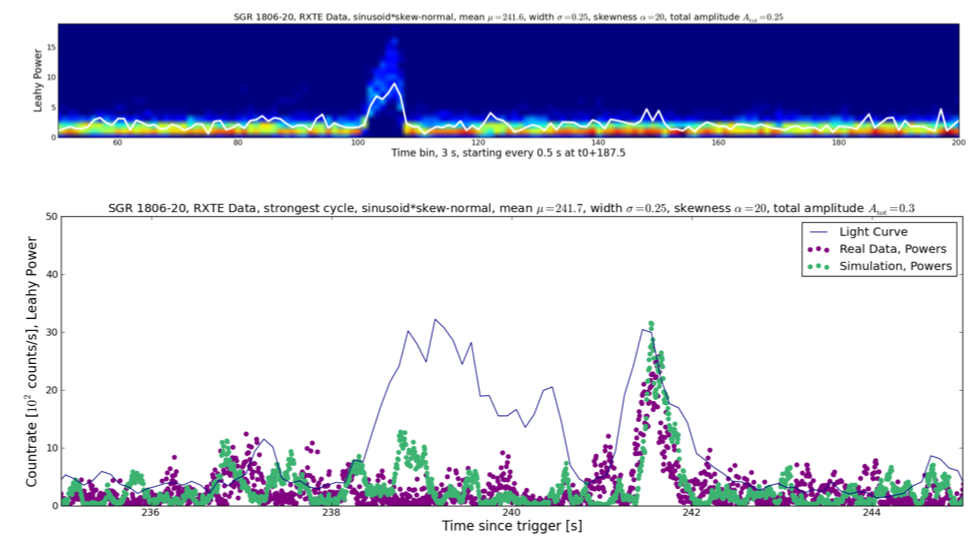
\includegraphics[width=\textwidth]{1806_rxte_lc_combined.png}
\caption{default}
\label{default}
\end{center}
\end{figure*}


There is a strong QPO signal at $625$ Hz in a cycle starting at $239\, \mathrm{s}$ after the trigger, as reported in \citet{Strohmayer06}. In order to answer the question whether this signal is present over all nine cycles, for which results are reported in \citet{Strohmayer05}, or whether it is only present in a single cycle, we constructed phase-averaged periodograms averaging up to nine periodograms, and constructed p-values as described in Section \ref{sec:analysis}. Figure \ref{fig:rxte_pvals} presents the results: the QPO is significant when averaging together up to $9$ cycles to $p < 0.02$. However, we also note that the signal is most significant when averaging the cycle with the strongest signal and the immediately previous cycle together. This indicates that the QPO is likely to be present at least in these two cycles. When averaging more than two cycles, the significance drops (the p-value rises, i.e. the null hypothesis, pure noise and no QPO, becomes more likely), indicating that with every additional cycle, we are averaging in more noise rather than more signal. We conclude that the signal is most likely present in two cycles at most.
We also note that we fail to reproduce the marginal detection of a QPO at the same frequency six cycles before the cycle with the strongest incarnation of the $625\, \mathrm{Hz}$ QPO. 

Given that the QPO is likely confined to two cycles, it is reasonable to ask whether the QPO extends over both cycles, i.e. is present for the entire $\sim 14\, \mathrm{s}$, or is being re-excited. To test this, we attempted to constrain the width of the QPO in the strongest cycle, in two ways. First, we redid the analysis described above, but with time segments starting exactly one cycle of the $625 \, \mathrm{Hz}$ QPO apart, i.e. every $1/625 = 1.6 \times 10^{-3} \, \mathrm{s}$ apart, effectively providing a finely resolved sliding window over the cycle where the QPO is strongest. If one then plots the strength of the signal with time, one can track the strength of the QPO over the course of the star's rotational cycle. As more signal is included in a given segment, the power will rise, until the entire signal is included. Similarly, as the sliding window moves out of the time frame where the QPO is located, less and less signal is included, and the power drops. We show the resulting plot in Figure \ref{fig:rxte_combined}. Similarly to Figure 3 in \citet{Strohmayer06}, the QPO seems to be present only on the declining edge of the second pulse, and only for a short period of time. We then injected an artificial sinusoidal signal into a single cycle in 50 simulations, in the same part of the rotational cycle as the real QPO, for a duration of $0.25\, \mathrm{s}$ and a fractional rms amplitude of $0.3$. The sinusoid is on top of a fast-rise exponential decay profile, to simulate the effect of a suddenly appearing, then decaying signal. We show a single realisation in the lower panel of Figure \ref{fig:rxte_combined}. In the upper panel, we show an image of the simulations, with data over plotted. The data traces the simulations as well, indicating that the observed QPO can be well modelled with a short, decaying, but high-amplitude QPO signal. 


\subsection{RHESSI}
\label{sec:rhessi_results}

\citealt{Watts06} searched segments of $t_{\mathrm{set}} = 2.27$ seconds length, i.e. $1/3$ of the neutron star's rotational cycle, over a range of 19 successive cycles, starting $\sim 80 \, \mathrm{s}$ after the onset of the giant flare. We varied the length of the segments between $0.5 \, \mathrm{s}$ and $2.0 \, \mathrm{s}$ in order to be sensitive to shorter signals, which may be buried in noise when taking the periodogram over too long a segment. We subdivided each cycle into $N_\mathrm{s} = 30$ segments, such that they start every $d t_\mathrm{set}= 7.6022/30 = 0.2534 \, \mathrm{s}$ apart, and overlap for $\delta t_\mathrm{set} - 0.2534 \, \mathrm{s}$.


TO ADD:
- periodogram of individual signal in strongest cycle
- show a savg example plot?
- pvalues
- simulation with similar p-values


\section{Discussion}
\label{sec:discussion}

\bibliography{bibliography}
\bibliographystyle{apj}

\end{document}
